\section{Исследовательская часть}

\subsection{Цель эксперимента}

Целью эксперимента является выявление зависимости времени выполнения запроса от числа записей в таблице, а также от вида самого запроса.

Чтобы достигнуть поставленной цели, требуется решить следующие задачи:
\begin{itemize}
	\item выбрать запросы, время выполнения которых будет замеряться;
	\item измерить время для каждого запроса и каждого числа записей в таблице;
	\item построить график зависимости времени от размеров таблиц и запросов;
	\item проанализировать полученные результаты.
\end{itemize}

Ниже приведены технические характеристики устройства, на котором будет проводиться эксперимент:
\begin{itemize}
	\item операционная система: Windows 10 64-bit Home;
	\item оперативная память: 8 GB;
	\item процессор: 11th Gen Intel(R) Core(TM) i3-1115G4 @ 3.00GHz \cite{intel}.
\end{itemize}

\subsection{Постановка эксперимента}

При эксперименте использовались запросы двух видов.

Первый вариант запроса:

\begin{lstlisting}
	select *
	from rehearsal join room on rehearsal.roomid = room.id
	join account on rehearsal.musicianid = account.id
	join reh_base on room.baseid = reh_base.id
\end{lstlisting}

Второй вариант запроса:

\begin{lstlisting}
	select rehearsal.rehdate, room.name, room.type, room.area, room.cost,
	reh_base.name, reh_base.address, reh_base.phone, reh_base.mail
	from rehearsal join room on rehearsal.roomid = room.id
	join account on rehearsal.musicianid = account.id
	join reh_base on room.baseid = reh_base.id
\end{lstlisting}

Число записей изменялось последовательно от 1000 до 10000 с шагом 1000. Каждый замер проводился по 100 раз, после чего вычислялось среднее время выполнения. Время измерялось в наносекундах с помощью функции 

perf\_counter\_ns() из библиотеки time.

\subsection{Результаты эксперимента}

По результатам измерений времени выполнения запросов можно составить таблицы \ref{tab:first} – \ref{tab:second} и диаграмму \ref{img:graph}.

\begin{table}[!h]
	\captionsetup{justification=centering}
	\caption{\label{tab:first} Результаты замеров времени выполнения 1-го запроса}
	\begin{center}
		\begin{tabular}{|p{0.06\textwidth}|p{0.06\textwidth}|p{0.06\textwidth}|p{0.06\textwidth}|p{0.06\textwidth}|p{0.06\textwidth}|p{0.06\textwidth}|p{0.06\textwidth}|p{0.06\textwidth}|p{0.06\textwidth}|p{0.07\textwidth}|}
			\hline
			Число записей & 1000 & 2000 & 3000 & 4000 & 5000 & 6000 & 7000 & 8000 & 9000 & 10000\\
			\hline
			Время & 5 350 973 & 8 883 559 & 13 577 113 & 19 818 492 & 21 778 098 & 26 708 169 & 32 112 573 & 35 606 740 & 40 054 833 & 46 621 729\\
			\hline
		\end{tabular}
	\end{center}
\end{table}

\clearpage

\begin{table}[!h]
	\captionsetup{justification=centering}
	\caption{\label{tab:second} Результаты замеров времени выполнения 2-го запроса}
	\begin{center}
		\begin{tabular}{|p{0.06\textwidth}|p{0.06\textwidth}|p{0.06\textwidth}|p{0.06\textwidth}|p{0.06\textwidth}|p{0.06\textwidth}|p{0.06\textwidth}|p{0.06\textwidth}|p{0.06\textwidth}|p{0.06\textwidth}|p{0.07\textwidth}|}
			\hline
			Число записей & 1000 & 2000 & 3000 & 4000 & 5000 & 6000 & 7000 & 8000 & 9000 & 10000\\
			\hline
			Время & 2 801 220 & 5 349 398 & 7 868 523 & 12 793 699 & 13 863 790 & 16 516 216 & 19 407 919 & 24 735 794 & 24 548 257 & 26 687 837\\
			\hline
		\end{tabular}
	\end{center}
\end{table}

\begin{figure}[h!]
	\begin{center}
		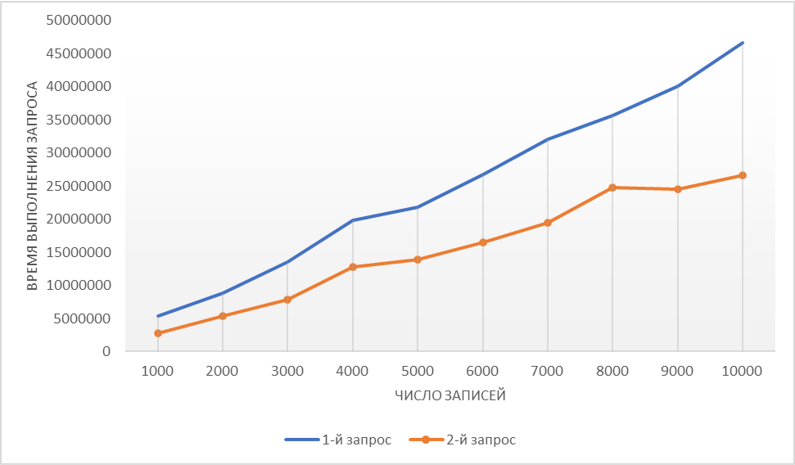
\includegraphics[scale=1.1]{inc/img/graph.png}
	\end{center}
	\captionsetup{justification=centering}
	\caption{\label{img:graph} Зависимость времени выполнения запросов от числа записей}
\end{figure}

%\clearpage

\subsection*{Выводы}
В данном разделе был проведён анализ времени выполнения двух видов запросов в зависимости от числа записей. 

В результате было выяснено, что время выполнения прямо пропорционально числу записей. Также было выяснено, что второй вариант запроса выполняется быстрее первого. За счёт усовершенствования запроса удалось снизить время выполнения в среднем примерно на 40,3\%.

Таким образом, на основании полученных данных можно сделать вывод, что на время выполнения запроса влияет как число записей в таблице, так и вид самого запроса.

